\def\year{2017}\relax
%File: formatting-instruction.tex
\documentclass[letterpaper]{article}
\usepackage{aaai17}
\usepackage{times}
\usepackage{helvet}
\usepackage{courier}
\usepackage{url} 
\usepackage{multicol}
\usepackage{array}

\usepackage{graphicx}
\graphicspath{ {images/} }

\usepackage[breaklinks=true]{hyperref}
\usepackage{breakcites}
\frenchspacing
\setlength{\pdfpagewidth}{8.5in}
\setlength{\pdfpageheight}{11in}
\pdfinfo{
/Title (Nasty, Brutish, and Short: 
What Makes Election News Popular on Twitter?)
/Author (Anonymous)}
\setcounter{secnumdepth}{0}  
 \begin{document}
% The file aaai.sty is the style file for AAAI Press 
% proceedings, working notes, and technical reports.
%
\title{Nasty, Brutish, and Short: 
What Makes Election News Popular on Twitter?}
\author{Anonymous\\
%Association for the Advancement of Artificial Intelligence\\
%2275 East Bayshore Road, Suite 160\\
%Palo Alto, California 94303\\
}
\maketitle
\begin{abstract}
AAAI creates proceedings, working notes, and technical reports directly from electronic source furnished by the authors. To ensure that all papers in the publication have a uniform appearance, authors must adhere to the following instructions. 
\end{abstract}

 
\section{Introduction}
In the changing landscape of both journalism and politics, social media is playing an increasingly large role in mobilizing and spreading information to citizens. A Pew Research survey from August 2015 showed that nearly two-thirds of adults in the U.S. who are on Twitter use the platform to get news \cite{pew-Twitter-news}. During the 2016 election year, the New York Times published an article estimating a 2 billion-dollar advantage in free media, including social media, for Donald Trump, all of which has no small impact on the messages broadcast to voters [13].

Although social media messages are less able to be carefully controlled in comparison to paid advertisements, they also have the potential to reach a wider audience. Reactions to an article shared by one potential voter now have the ability to be broadcast and spread to millions of others in a real-time, public sphere. 

%Measuring the way that stories grow and spread has become an important part of the equation to understanding public discourse.

The popularity of sharing articles on social media also marks an important shift in the role of the news consumer from armchair reader to information propagator. Whereas news used to be broadcast to the reader, now each reader has the potential to broadcast stories to his or her own audience. Sharing a story requires a level of interest and activation on the part of the reader beyond simply reading a story; yet often, this trigger is predictably emotional in nature. 

In a 2011 study of the New York Time’s ``most emailed list'', Berger and Milkman found that the potential for a news story to go viral is partially driven by physiological arousal, defined as ``an excitatory state of sensory alertness, mobilization, or energy'' [Milkman 7]. In short, the desire to share a certain story is often universally impulsive, regardless of context. Yet in the case of political news, this impulse can have a large impact on reach of political messages.
 

 \subsection{Hypotheses}
With the impact of social media in politics  \emph{and} the often emotionally charged nature of content-sharing in mind, we ask the following question in our research: 

\begin{itemize}
\item Does the emotional vocabulary of political news stories have an impact on its Twitter popularity that persists beyond political affiliation?  
\end{itemize}

To test this question, we focus on three key aspects of stories: length, emotionality, and positivity, based on behavioral theories of the Internet and studies of political news detailed in the section below.  

We hypothesize the following behavior in our dataset of stories and tweets:

\begin{itemize} 
    \item \textbf{H1:} Story length has a \emph{negative} correlation with Twitter shares, due to the effects of the Internet attention economy and overexposure to political media \cite{goldhaber1997attention}.
    \item \textbf{H2:} Emotionality has a \emph{positive} correlation with Twitter shares, consistent for viral content in general \cite{berger2012makes}.
    \item \textbf{H3:} Positivity has a \emph{negative} correlation with Twitter shares, due to the nature of political news and contrary to generalized findings \cite{berger2012makes}

\end{itemize}

For each of these three independent variables (story length, emotionality, positivity) we repeat analyses across three views of the data: first, the entire dataset; then, by political candidate followed amongst users who follow only one candidate; and finally, by the number of political candidates followed (degree of political engagement), to look for differences amongst different populations of political tweeters.


\section{Literature Review}
% \subsection{The Social Media Megaphone}
% In the changing landscape of both journalism and politics, social media is playing an increasingly large role in mobilizing and spreading information to citizens. President Barack Obama’s win in 2008 is often attributed as the first example of a successful social media campaign in the elections. Establishing an online presence that recruited more than 3 million individual contributors and 5 million volunteers, Obama created a grassroots political movement \cite{cogburn2011networked}. Publicity and public sound bites matter-- especially when it’s free and has the potential to go viral.

% This election cycle, in particular, already shows a heavy skew by social media. The New York Times estimated a 2 billion-dollar advantage in free media for Donald Trump on platforms from television to Twitter, all of which has no small impact on the messages broadcast to voters \cite{nyt-trump-free-media}. Although ``free media'' messages have less ability to be carefully controlled in comparison to paid advertisements, they also have more potential to reach a wider audience. Sentiments echoed by one potential voter now have the ability to be broadcast and spread to millions of others in a real-time, public sphere.
  
\subsection{The (Short) Attention Economy}
At the same time that social media has the power to create a flood of free advertising and media for political candidates, the abundance of information on the web has created new challenges and questions about the kind of content being processed by readers. This paradox-- between the ease of accessibility to information and the increasingly limited bandwidth of consumers-- is described as one of the challenges of being in an \emph{attention economy} \cite{goldhaber1997attention}. Moreover, high-impact events like the presidential elections especially intensifies this effect-- about 60 \% of Americans reported feeling exhausted by media coverage of the elections in July of 2016 \cite{election-fatigue}. To explore the effects of the attention economy on the reading of political news, we examine story length and how it relates to sharing popularity in the analysis to follow.
 

\subsection{Negativity in Politics and the Internet}
In addition, the option of anonymity and pseudo-anonymity on a social network like Twitter (along with other traits of Internet communication), is theorized to contribute to increased negative and hostile behavior, potentially increasing tension for the already-fraught subject of politics. This phenomenon, is coined as the \emph{online disinhibition effect} \cite{suler2004online}. 

In Berger and Milkman’s study of story virality, it was found that \emph{positive} content was more likely to be shared than negative content-- against conventional belief \cite{berger2012makes}. Political news, however, is a unique category of news, and this election in particular-- where one-in-four Americans report disliking the presidential candidates-- appears to have a negative overtone.

To compare the sharing of election news stories versus patterns of general virality in the news, and to examine the extent in which negative sentiment is popular, we calculate the \emph{negativity} of stories, and how that relates to Twitter behavior.

We also examine the effects of the degree of combined emotionality in the content and how that relates to Twitter shares, to see if either more positive or more negative content is more likely to be shared overall than content that ranks low in emotionality. Although positive content was found to be more popular than negative content in the sharing of stories, both highly positive and highly negative content was more likely to become viral, and we expect the same to hold for political news \cite{berger2012makes}. 
 
\section{Data Collection}
 Our main dataset is a connected corpus of news articles about the presidential elections and the tweets that share them from January 1, 2016 to May 1, 2016 over 13 news outlets. In this chapter, we detail the collection and creation of our dataset, along with the unique challenges of working with ``big data''.

\subsection{The Electome Project}
The backbone of our data collection and classification process lies under the umbrella of the Electome project, a large, collaborative effort with the Laboratory for Social Machines to examine the ``horse-race of ideas'' and competition of narratives during the presidential election year. The goal of the Electome project is to create novel stories for data journalists as well as technically innovative ways to examine the national conversation using machine learning and ``big data'' analysis through both social and traditional media coverage. The first step of both our news and Twitter data processing method uses machine learning classifiers from the Electome project.

\subsection{News Dataset}

 \subsubsection{Duration \& Scope}
 For our news dataset, we scraped articles from the RSS feeds of news publications every hour over five months and 13 publications:

\begin{multicols}{2}
\begin{itemize}

\item CNN
\item Fox News
\item The New York Times
\item The Wall Street Journal
\item The Washington Post
\item The Los Angeles Times 
\item The Associated Press
\item Reuters
\item McClatchy 
\item Politico 
\item Buzzfeed
\item The Huffington Post
\item NPR 
\end{itemize}
\end{multicols}

The choices above span a mix of publications. We include sources that: 

\begin{itemize}
\item Have mostly conservative audiences and mostly liberal audiences \cite{PoliticalPolarization}
\item Come from mixed primary media formats (television, paper, online, radio)
\item Are viewed as ``legacy'' (over a hundred years old) and ``new'' media (founded online within the last 10 years)
\item Focus solely on political news (Politico, McClatchy)
\item Are newswire services (the Associated Press, Reuters news)
\end{itemize}
 
 to capture a variety of types of election coverage and target audiences.
 
 We look at stories from January 1, 2016 (the start of the election year) to May 1, 2016. This time period captures the bulk of the primary election, when coverage of multiple presidential candidate contenders creates greater variety in news stories for our analysis.
  
\subsection{Data Pipeline}

Articles are processed in a 3-step pipeline, pictured below.


\begin{figure}[t!]
\centering
%\includegraphics[width=\columnwidth, page=33, trim = 0mm 71mm 190mm 66mm, clip=true]{presentation} 
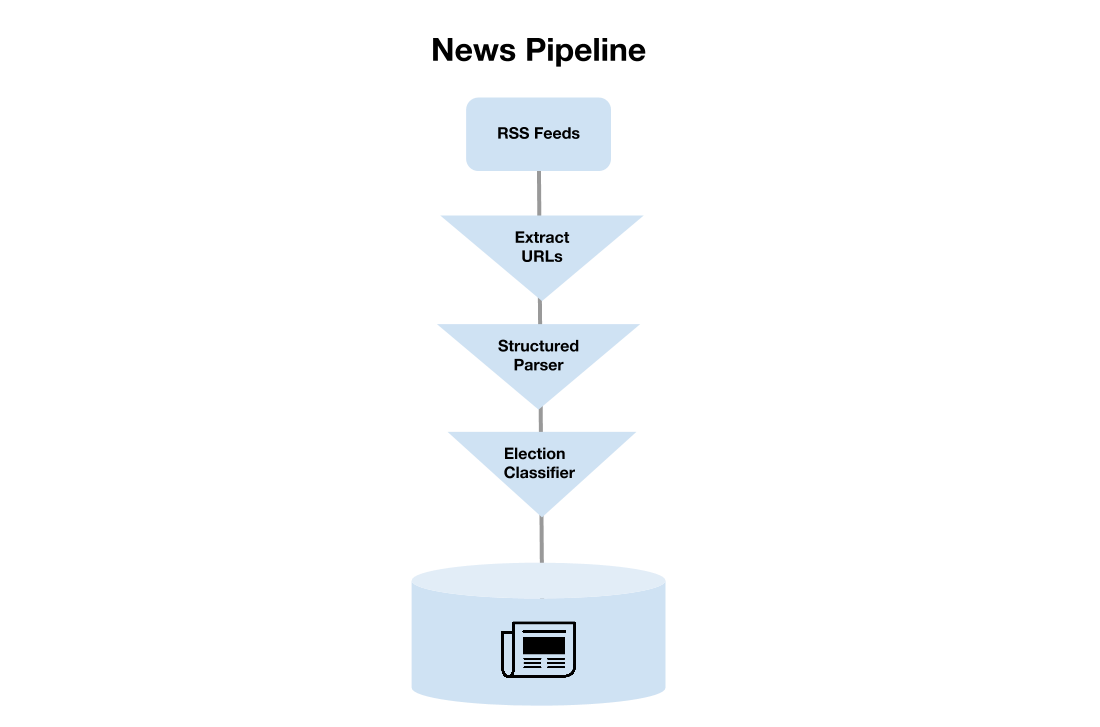
\includegraphics[width=\columnwidth]{election-news-pipeline}  
\caption{Election News Pipeline
     \label{fig:data-stack}}
\end{figure}

% \begin{figure} %[H]  
% \centering 
%   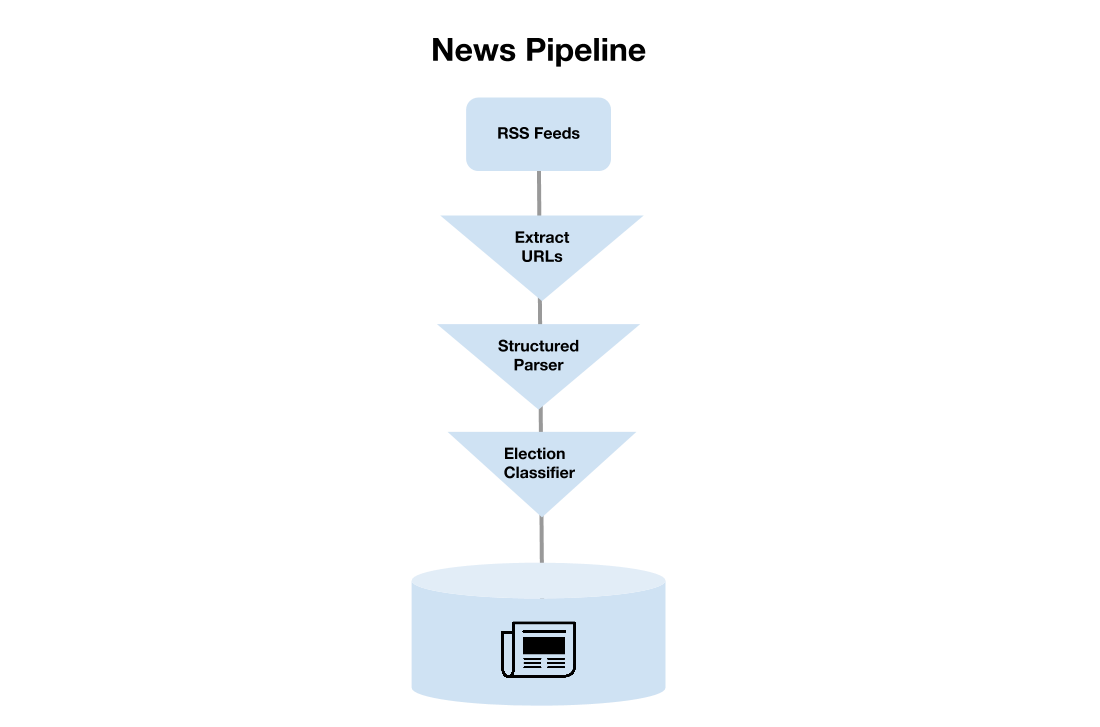
\includegraphics[width=0.9\textwidth]{election-news-pipeline}  
%   \caption{Election News Pipeline
%     \label{fig:data-stack}}
% \end{figure}

After collecting the links to the full content of the news stories from each publication's RSS feed, we pass each link to a structured content parser that extracts entities and features from the raw HTML.

The story text is then passed into a machine learning classifier for election news from the Electome project \footnote{Designed and implemented by Prashanth Vijayaraghavan.}. 


 We collect and classify a total of 22,959 articles as election-related with over 80\% confidence, an average of 5,700 per month and 191 per day.


\section{Tweets Dataset}

\subsection{Duration \& Scope} 
The Laboratory for Social Machines was founded on the premise of a research grant with Twitter which allows access to the ``firehose'' of all activity on Twitter. We start with the pool of all tweets between January 1, 2016 and May 1, 2016 in our data process.

\subsection{Data Pipeline}

Tweets pass through a similiar pipeline as news stories. We sort all tweets with an election classifier which has been shown to be able to detect election-related tweets with an F-score of 92\% \cite{vijayaraghavan2016automatic}. We then filter by those that share a link (which might potentially be a news story).

\begin{figure}[t!]
\centering
%\includegraphics[width=\columnwidth, page=33, trim = 0mm 71mm 190mm 66mm, clip=true]{presentation} 
\includegraphics[width=\columnwidth]{Twitter-pipeline}  
\caption{Election Tweets Pipeline
     \label{fig:data-stack-Twitter}}
\end{figure}


% \begin{figure} %[H]  
% \centering 
%   \includegraphics[width=0.5\textwidth]{Twitter-pipeline}  
%   \caption{Election Tweets Pipeline
%     \label{fig:data-stack-Twitter}}
% \end{figure} 

We collect and sort a total of 16,667,685 tweets as election-related and containing at least one URL in the text, an average of 4,000,000 per month and 140,000 per day.

\section{Combined Dataset}
The final step of our data collection process is to extract, expand and connect the links shared in our election-related tweets with articles in our database.
 
\subsection{Mapping Tweets to Stories}

\begin{figure}[t!]
\centering
%\includegraphics[width=\columnwidth, page=33, trim = 0mm 71mm 190mm 66mm, clip=true]{presentation} 
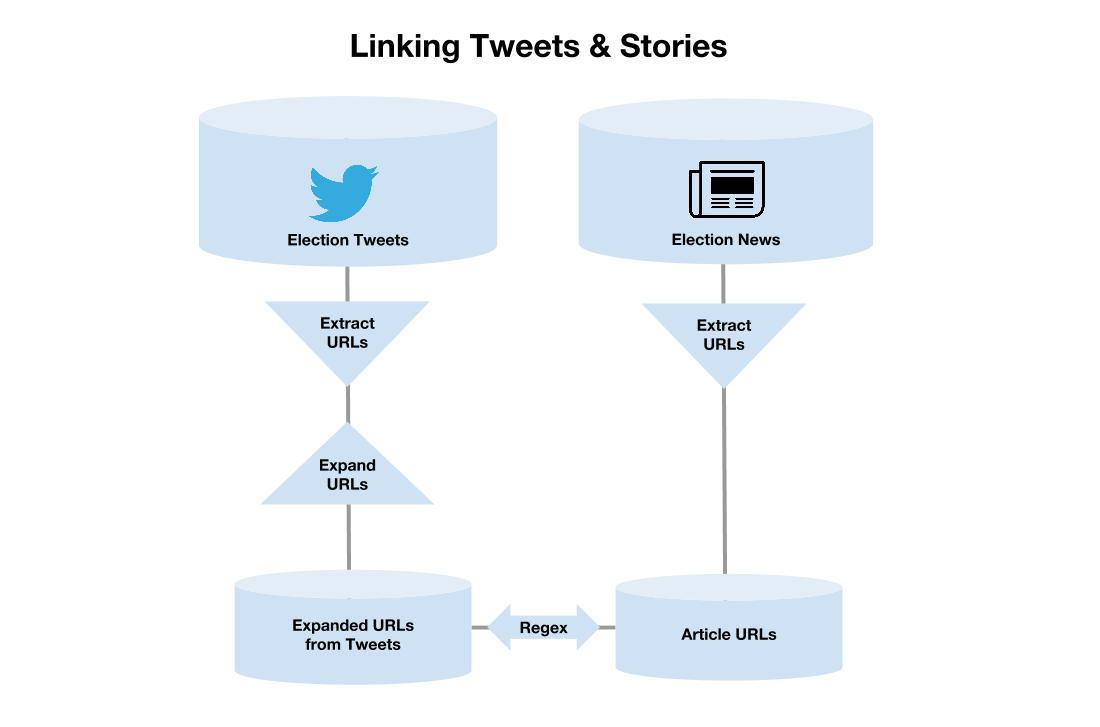
\includegraphics[width=\columnwidth]{data-stack} 
\caption{Data Pipeline}
\label{fig:data-stack}}
\end{figure}

% \begin{figure} %[H]  
% \centering 
%   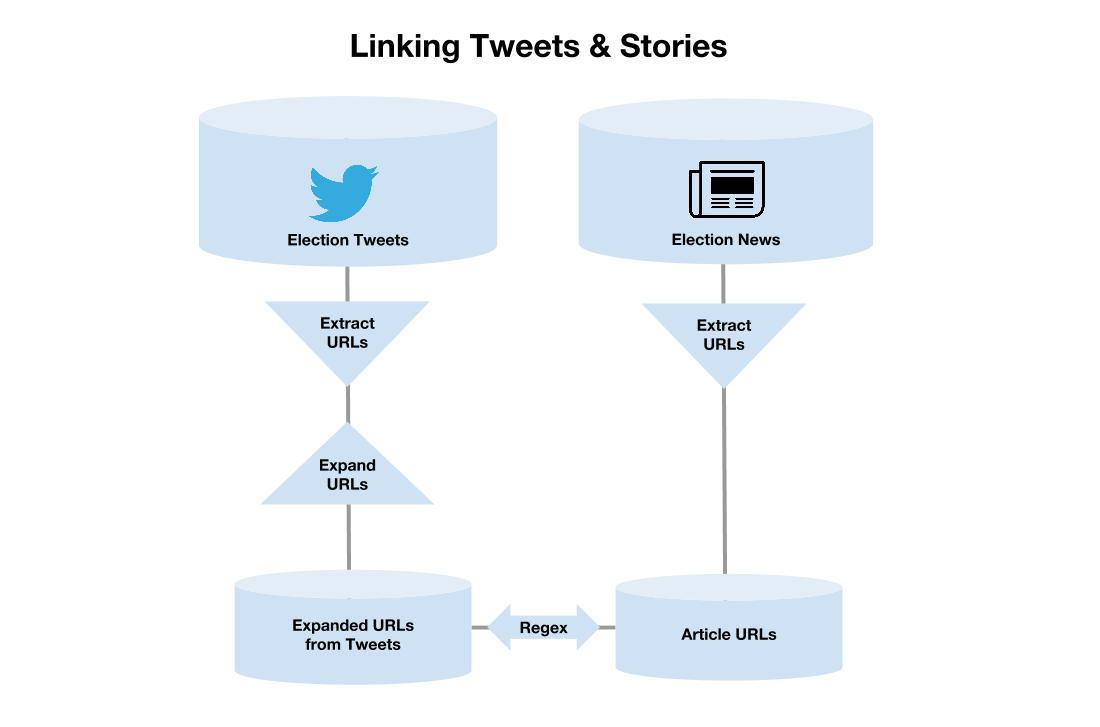
\includegraphics[width=0.5\textwidth]{data-stack}  
%   \caption{Data Pipeline
%     \label{fig:data-stack}}
% \end{figure}
 
Twitter automatically formats all links into a shortened ``t.co'' format, so we first expand all links in tweets (16.6 million), then use a regular expression to see if the final destination of the expanded link matches a query-truncated URL of a story in our database. We checked the validity of 382 billion url-story matches in less than a day by running the processes on the Amazon Web Services cloud computing platform in parallel using the Gnu-parallel command line tool \cite{tange2011gnu}.

\subsection{Final Corpus}

In total, we found that 30\% of the election stories we tracked were shared on Twitter during the time period of January 1st through May 1st.

There were 137,986 tweets that contained a link to 6,911 unique stories (out of 22,960).

Since we chose the story to be the unit of analysis in this thesis, we then eliminated any stories that were shared by less than 10 tweets.

This left a total of 2,650 distinct articles (38\%) shared in 123,113 (89\%) tweets by 20,956 Twitter users (93\%).

\subsection{Descriptive Findings}
%Of the 2,658 articles shared 123,133 times on Twitter that we track in our studies, the vast majority are shared less than 100 times. 
The vast majority of stories are shared less than 100 times. 

\begin{figure}[t!]
\centering 
  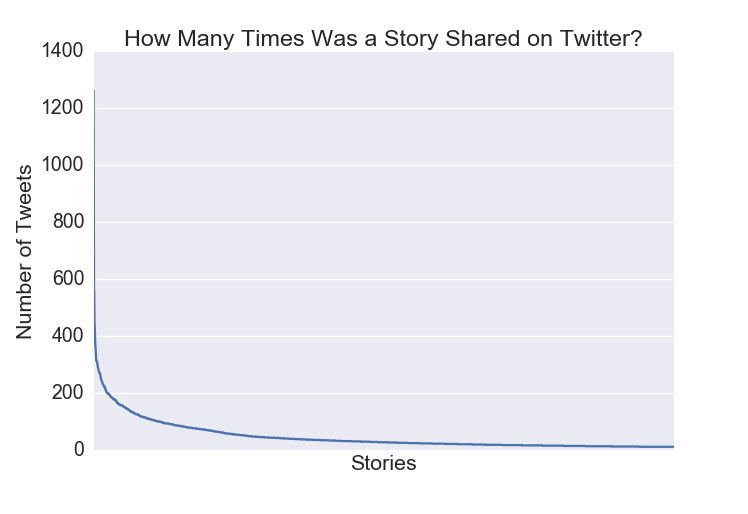
\includegraphics[width=\columnwidth]{story-share-dist}  
  \caption{Distribution of Story Shares
    \label{fig:story-share-dist}}
\end{figure} 



Story sharing behavior follows an approximate power law distribution. On average, stories are shared 46 times, however, the median (50th percentile) of shares is just 26. 


CNN, Politico, and Fox lead in publication popularity with the highest number of stories shared by tweets in our dataset-- likely due to the volume and close association to political content of the companies. Because our data pipeline detailed in the previous chapter looks for election-related news, outlets which track the campaign extensively are more likely to show up in our results.


\begin{figure}[t!]  
\centering 
  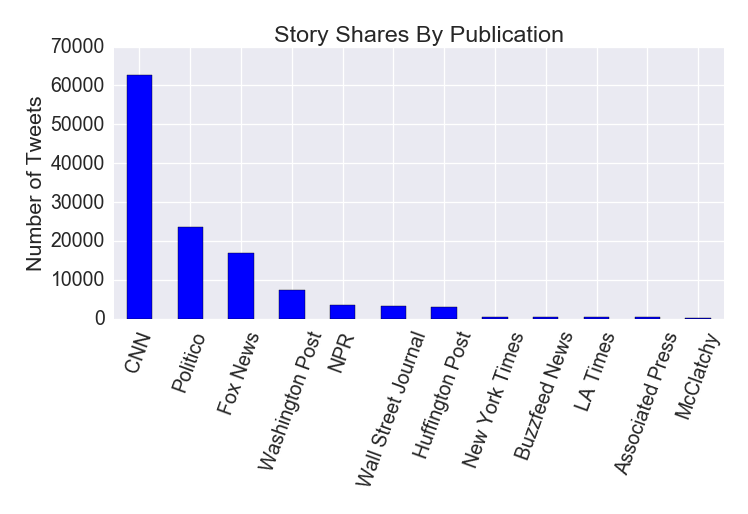
\includegraphics[width=\columnwidth]{all-stories-by-pub}  
  \caption{Number of story shares by publication
    \label{fig:tweets-by-pub}}
\end{figure} 


\newpage %force table to get on the next page

Examining the top 10 most shared stories, it comes as no surprise that outsized personality Donald Trump is by far the most ``tweetable'' candidate, dominating the list with 7 out of 10 stories featuring his name in the title.

 
\begin{table}
%\begin{tabular}{| l || c |} 
\begin{tabular}{ |l c| } 
    %s\toprule
    \hline
    Article &  \# tweets \\
    \hline
    %\midrule
    The One Weird Trait That Predicts Whether You're a Trump Supporter &   1260 \\
    Donald Trump Is Shocking, Vulgar and Right                         &    901 \\
    Biden praises Sanders on income inequality                         &    563 \\
    Why I'm voting for Trump                                           &    554 \\
    Anne Frank's stepsister compares Donald Trump to Adolf Hitler      &    445 \\
    Trump basks in his spotlight                                       &    436 \\
    Rubio: Law-abiding undocumented immigrants could stay              &    413 \\
    Terrorists use Trump's `Muslim ban' speech in recruitment video    &    398 \\
    Iowa caucuses: Donald Trump's moment of truth                      &    364 \\
    GOP senators: If Cruz wins, we lose                                &    357 \\
    %\bottomrule
    \hline
\end{tabular}
\caption{\label{tab:top-10}Top 10 Shared Stories}
\end{table}

\begin{figure}[t!]  
\centering 
  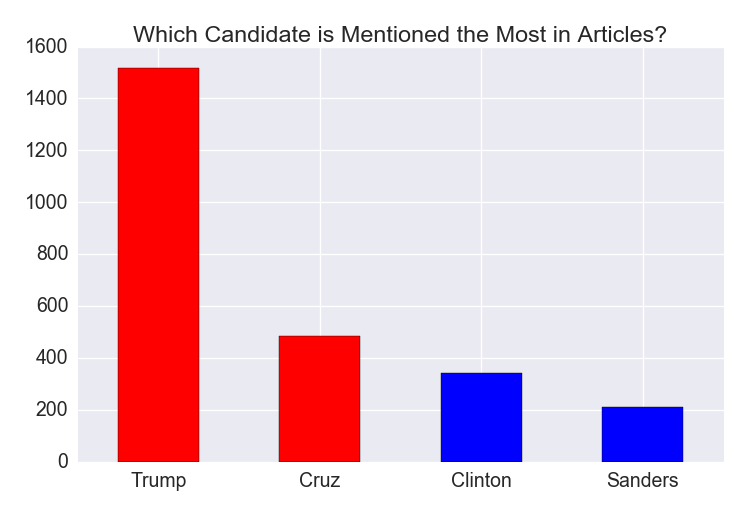
\includegraphics[width=\columnwidth]{candidate-mentions}  
  \caption{Most frequently mentioned candidate in stories
    \label{fig:tweets-by-pub}}
\end{figure} 


The \emph{extent} to which he is prominent in articles is clear: by coding each story by the most frequently mentioned candidate, Trump has nearly three times as much coverage at nearly 60\% as the runner-ups, Ted Cruz and Hillary Clinton.

The large number of stories with Cruz as the most-mentioned candidate are likely due to his association to Trump as a Republican runner-up: 96\% of stories where Cruz is the most-mentioned candidate feature Trump as the second-most frequently occuring.
 





\bibliographystyle{aaai} \bibliography{nasty-brutish-short.bib}

\end{document}
